\section{母模型风险、备用与场景压缩对照}
\label{app:optional_models}

本附录集中列示未启用候选筛选的母模型扩展。正文采用28场景、零附加风险和零参考备用；以下实验保留各自原配置。

\subsection{风险与备用的可选扩展}

经济主案取$\lambda=\rho_t=0$。为识别额外保守程度的影响，对照在式\eqref{eq:q2_objective}加入$\lambda\operatorname{CVaR}_{0.90}(Q)$，其损失对象$Q$为场景紧急费用。按照文献\cite{rockafellar2000}写为
\begin{equation}
 \begin{cases}
 \displaystyle
 \operatorname{CVaR}_{\alpha}(Q)=
 \min_{z,\{v_s\}}\left\{z+\frac{1}{1-\alpha}\sum_s\pi_sv_s\right\},\\
 v_s\ge Q_s-z,\\
 v_s\ge0,\\
 \alpha=0.90.
 \end{cases}
 \label{eq:cvar}
\end{equation}
自适应权重根据近期残差总体标准差设定：
\begin{equation}
 \begin{cases}
 \lambda=0.10\min\{3,r/0.20\},\\
 \displaystyle r=\frac{\operatorname{mean}_t\operatorname{sd}_j(\epsilon^n_{j,t})}
 {\max\{\operatorname{mean}_t|\widehat n_t|,50\}}.
 \end{cases}
 \label{eq:risk_weight}
\end{equation}
标准差分母取历史样本日数，50 kWh用于稳定净需求接近零时的比值。固定风险权重取一月自适应序列均值0.10368，之后保持不变。

参考备用沿同一历史日累加未来至多六段误差，以外侧累计缺口换算为内部库存：
\begin{equation}
 \rho_t^{\rm raw}
 =k_\rho\min\left\{2400,
 \frac{\left[q_{0.8}\left(\sum_{k=t+1}^{\min(t+6,143)}
             \epsilon^n_{j,k}\right)\right]_+}{\eta_d}\right\},
 \label{eq:reserve}
\end{equation}
\begin{equation}
 \begin{cases}
 \rho_t=\min\{\rho_t^{\rm raw},
 [e_\tau-E_{\min}+\eta_cU(t-\tau+1)]_+\},\\
 e_{t+1}\ge E_{\min}+\rho_t.
 \end{cases}
 \label{eq:reachable_reserve}
\end{equation}
问题二取$\tau=0$，滚动问题可取其他发布时点。分位数按排序样本间线性插值，空和为零；依次在2400 kWh截断、乘无量纲$k_\rho$，再按当前电量及最大充电速度作可达截断，缩放后的上限为$2400k_\rho$。

动态备用对照取$k_\rho=1$；固定备用取一月可达截断前动态备用均值208.67 kWh，日末置零，再作相同可达截断。一月匹配按每次外层更新实际覆盖的时段计数。备用约束外层参考轨迹，实际执行器仍可为当期负载使用该电量，并遵守1200 kWh物理下限。终端系数$\beta_T$单位为元/kWh，备用系数$k_\rho$无量纲。

\subsection{风险、备用及其联合作用}

\begin{table}[htbp]\centering\small
\caption{问题2风险与备用的完整对照}
\label{tab:v2_risk_modules}
\begin{tabularx}{\linewidth}{LRRRR}\toprule
策略 & 总费/万元 & 紧急量/kWh & 日费CVaR95/元 & 末库存/kWh\\\midrule
期望费用 & 1401.28 & 85017.69 & 70731.74 & 6240.32\\
固定风险 & 1411.84 & 56316.17 & 69028.62 & 6318.65\\
自适应风险 & 1405.41 & 66920.81 & 69476.71 & 6255.33\\
固定备用 & 1401.09 & 74987.90 & 70409.51 & 6240.32\\
动态备用 & 1402.30 & 76168.28 & 70299.39 & 6245.11\\
固定风险+备用 & 1413.36 & 49102.47 & 68862.93 & 6318.65\\
自适应风险+备用 & 1406.93 & 59081.98 & 69070.96 & 6260.12\\
自适应联合，12场景 & 1404.26 & 75336.25 & 70065.84 & 6289.57\\
\bottomrule\end{tabularx}
\par\smallskip\parbox{\linewidth}{\footnotesize 未启用候选筛选的母模型对照；各组沿用原实验配置，覆盖334天并连续推进状态。}
\end{table}

\begin{table}[htbp]\centering\small
\caption{固定与自适应策略在评价期实现的平均保守程度}
\label{tab:v2_conservatism}
\begin{tabularx}{\linewidth}{LRR}\toprule
策略 & 平均风险权重 & 平均参考备用/kWh\\\midrule
固定风险 & 0.10368 & 0.00\\
自适应风险 & 0.05506 & 0.00\\
固定备用 & 0.00000 & 207.22\\
动态备用 & 0.00000 & 244.39\\
固定联合 & 0.10368 & 207.22\\
自适应联合 & 0.05506 & 244.39\\
\bottomrule\end{tabularx}
\par\smallskip\parbox{\linewidth}{\footnotesize 固定参数按一月动态序列均值匹配，评价期保留该参数，报告季节变化下实现的平均值。}
\end{table}


与主案相比，仅固定风险增加105631.25元，仅自适应风险增加41280.51元，紧急量分别降至56316.17和66920.81 kWh。固定备用单独使用节省1891.73元，动态备用单独使用增加10152.11元，说明经济效果随备用形状和时段作用变化。联合自适应策略增加56524.93元，紧急量降至59081.98 kWh。表中CVaR95按实际日总账单计算。

评价期固定和自适应的平均风险权重分别为0.103681与0.055059，参考备用均值分别为207.22与244.39 kWh。虽然固定参数由一月均值匹配，两类方法在评价期的差异仍同时包含平均保守程度与时段分配的变化。

以$C_{\rm joint}-C_{\rm risk}-C_{\rm reserve}+C_{\rm expectation}$描述联合作用，固定和自适应两组分别为17088.03元和5092.30元，均为正，即本次闭环回测的联合费用高于两项单独费用变化的简单相加。

\begin{figure}[htbp]\centering
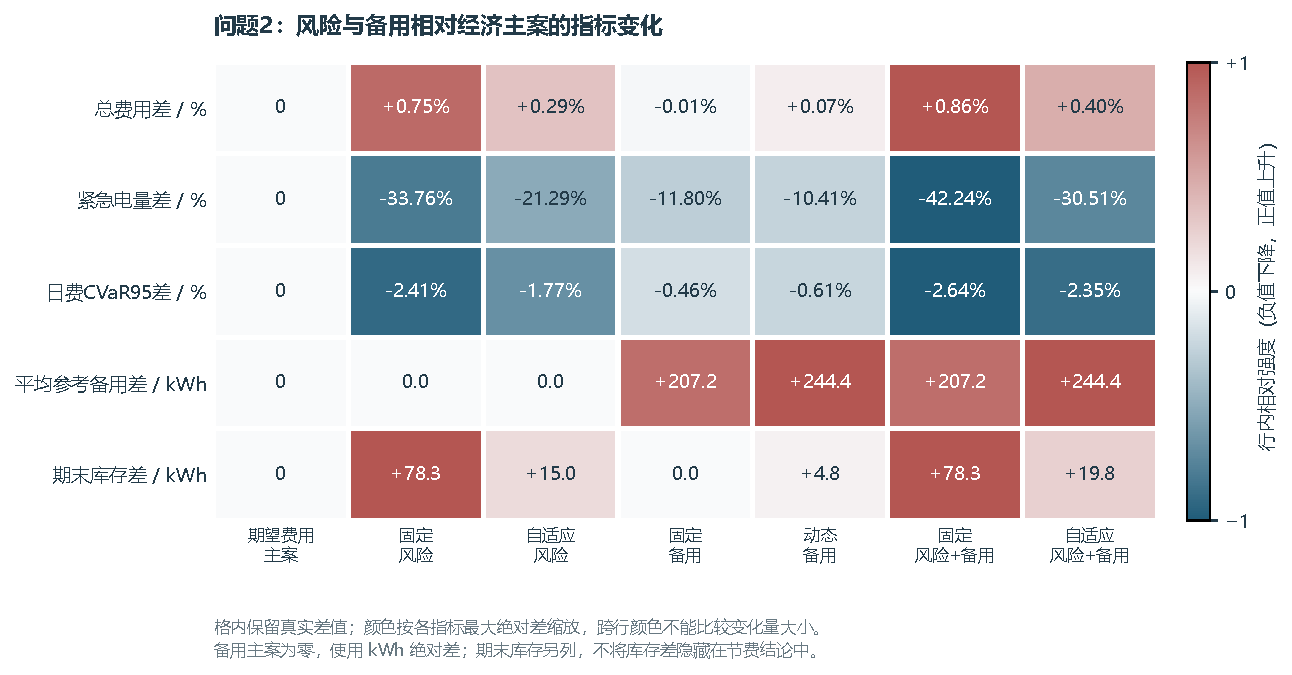
\includegraphics[width=0.95\linewidth]{figures/results/q2_risk_heatmap.pdf}
\caption{七种风险与备用设置相对主案的指标差异；前三行标注百分比，备用和末库存标注kWh差值，颜色仅在同一指标行内比较}
\label{fig:q2-risk-heatmap}
\end{figure}

图\ref{fig:q2-risk-heatmap}显示紧急购电减少往往伴随额外常规承诺。费用、紧急量和日费CVaR95用相对主案百分比表示；参考备用的主案值为零，故与末库存一样报告kWh差值。颜色按各指标行的最大绝对变化归一。主案保留冻结设置，风险扩展用于衡量减少补购需求的费用代价。

\subsection{28轨迹保留与12代表日压缩}

% Generated by code/make_question_tables.py; do not edit values.
% Source: data/experiments_v2.json; SHA256=e231ea14b234bd4593ec19c5f913ce028ed3b15ee677b4b58eafc7d3a658f29a
\begin{table}[htbp]\centering\small
\caption{问题二完整场景与压缩场景的同条件比较}
\label{tab:v2_scenarios}
\label{tab:v2_solve_times}
\begin{tabularx}{\linewidth}{LRRRR}\toprule
场景数 & 总费/万元 & 紧急量/kWh & 日费CVaR95/元 & 秒/日\\\midrule
28 & 1401.28 & 85017.69 & 70731.74 & 0.0521\\
12 & 1400.63 & 105407.24 & 72139.66 & 0.0276\\
\bottomrule\end{tabularx}
\par\smallskip\parbox{\linewidth}{\footnotesize 相同334天、预测、执行器及期初库存；末库存分别为6240.32和6257.26 kWh。时间包含预测、求解和执行，在本机并行条件下仅反映工程量级。}
\end{table}


经济目标下12场景比28场景少付6465.72元，却多购20389.55 kWh紧急电量，日费用CVaR95也更高。风险与备用联合开启时，12场景总费用14042623.21元、紧急量75336.25 kWh；28场景为14069332.59元、59081.98 kWh，体现了压缩对费用、尾部和紧急需求的共同影响。

28个等权历史日的10\%尾部对应2.8条轨迹的概率质量，压缩还会将其集中到少数代表日。主案按预定配置保留全部28条历史轨迹，求解耗时适合本题规模。

为核对缩减程序的数值过程，另外记录334个日期窗口的实际medoid迭代。令标准化历史轨迹为$x_j$，第$m$轮代表集合为$\mathcal M^{(m)}$，压缩距离目标为
\begin{equation}
 J_m=\frac{1}{|\mathcal H_D|}\sum_{j\in\mathcal H_D}
       \min_{\ell\in\mathcal M^{(m)}}\|x_j-x_\ell\|_2.
 \label{eq:q2_compression_objective}
\end{equation}
图\ref{fig:q2-scenario-convergence}将各窗口目标归一为$J_m/J_0$，显示跨窗口中位数和P10--P90经验分位区间。334个窗口均达到代表稳定，迭代次数中位数2、最大5，最终相对目标中位数0.9816002。代表和权重已逐窗口与原缩减函数输出核对。

\begin{figure}[htbp]\centering
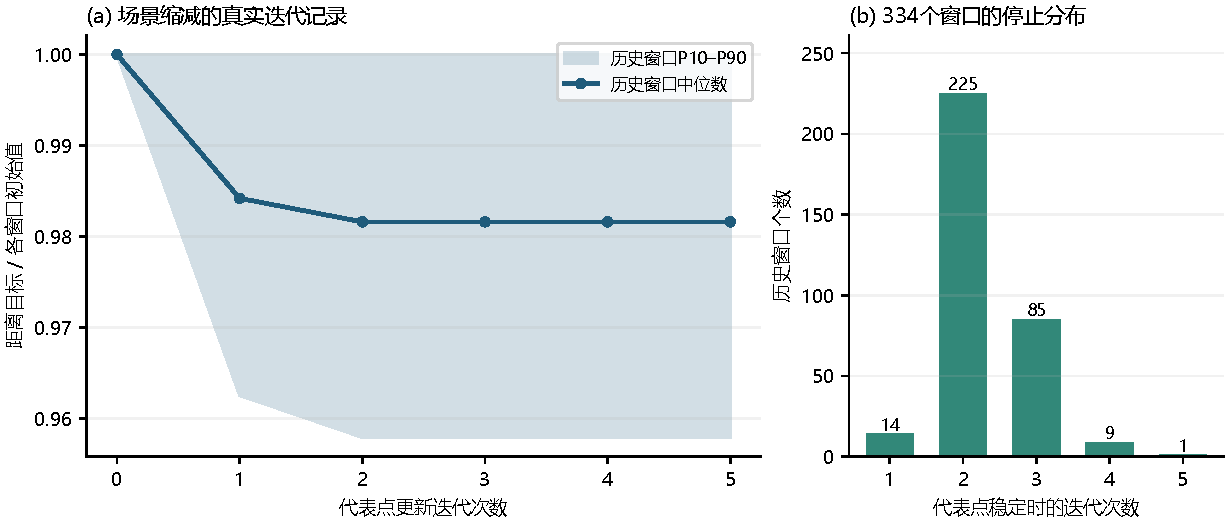
\includegraphics[width=0.93\linewidth]{figures/results/q2_scenario_convergence.pdf}
\caption{12代表日压缩距离目标的实际迭代；曲线为334窗口归一目标中位数，阴影为逐轮P10--P90经验分位区间}
\label{fig:q2-scenario-convergence}
\end{figure}

已停止窗口重复终值以对齐横轴，经验分位区间描述窗口间离散程度。该图核对历史轨迹的几何压缩过程，经济效果见表\ref{tab:v2_scenarios}及实际执行账单。
\FloatBarrier
